In all the following comparisons between the black box and the physics guided
network, the two have the exact same topology, are initialized to identical
states, and have identical inputs. The cost function is calculated identically
as well. The only difference is the addition of the physics prior.

\begin{figure}
	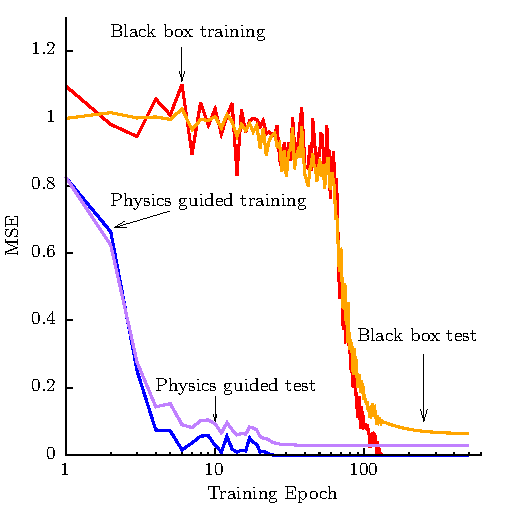
\includegraphics{figures/4-site-gs-mse.pdf}
	\caption{\textbf{Efficacy of physics guided training on learning} The lines 
	plot the mean square error for both the physics guided training 
 	and the black box training as a function of training epochs. 
	It is clear that for the exact same network topology, the 
	physics guided learning achieves better performance with 
	less exposure than the black box.}	
	\label{4-site-gs-mse}
\end{figure}

Figure~\ref{4-site-gs-mse} shows the mean square error as a function of training
epochs during the training phase for a four site generalized Ising ring with 
infinitesimal longitudinal field, and varying transverse field. The training 
data lies exclusively in the ferromagnetically ordered phase, whilst the 
testing data contains points in both the ferromagnetic phase and the 
disordered phase. The training and testing datasets are composed of strictly 
mutually exclusive samplings of the phase diagram. The inputs to the network 
are the elements of the Hamiltonian operator, and the output is the 
ground state wavefunction. What can be noticed in Fig~~\ref{4-site-gs-mse} is 
that the learning happens much faster in the physics guided model than in the 
black box model. Concomitantly the final mean square error is lower in the 
physics guided than in the black box. This is surprising given the two 
networks are more the same than different. 


\begin{figure}
	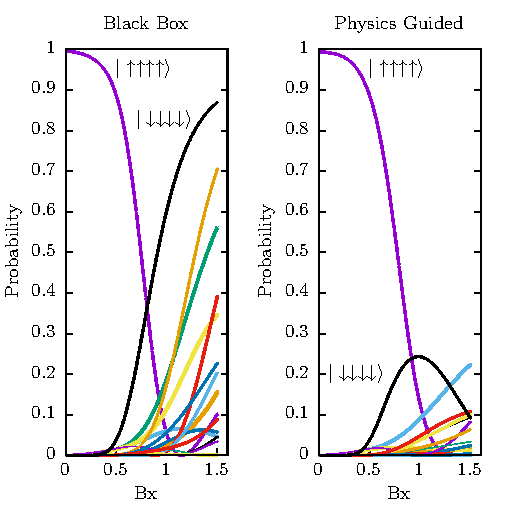
\includegraphics{figures/4-site-gs-coeff.pdf}
	\caption{\textbf{Efficacy of physics guided training on predictions} 
	The line plot the square of the coefficients of the ground state 
	wavefunction, representative of the probability of obtaining 
	a certain magnetic order. Across the phase transition boundary $B_x = 1$, 
	the physics guided machine makes better predictions.}	
	\label{4-site-gs-coeff}
\end{figure}


Figure~\ref{4-site-gs-coeff} shows the predictions of the square of the
coefficients of the ground state wavefunction. The lines plot each of the
coefficients as a function of increasing longitudinal field. The transverse
field Ising chain is known to have a quantum phase transition as a function of
transverse field strength at $B_x = 1$, if the energy scale is set by the Ising
coupling $J = 1$.  Here the magnetization of the model is determined by the
difference in the square of the first coefficient less the sixteenth. The
transition is identified by going from finite magnetization to zero
magnetization. In the left panel, with learning unguided by a prior, the
magnetization becomes zero near $B_x = 0.7$. In the right panel, the
magnetization dies out near $B_x = 0.9$.  This is already an improvement
towards predicting the thermodynamic limit, but is not the most important
feature. Comparing the physics guided to the unguided model, the physics guided
correctly identifies that the probability of obtaining an ordered state should
go to zero across the transition, whereas the unguided model has no such
inkling. Additionally, the physics guided machine more correctly preserves the
normalization condition, that the sum of the squares of the coefficients should
be one.  The black box machine completely violates this. 

\begin{figure}
	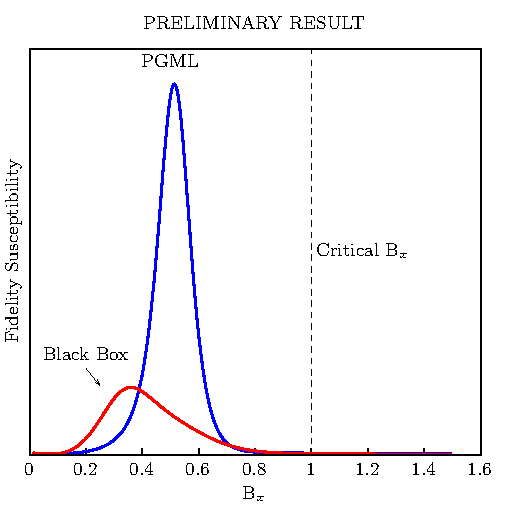
\includegraphics{figures/4-site-fidelity-susceptibility.pdf}
	\caption{\textbf{Efficacy of physics guided training on quantum observable} 
	The line plot the quantum fidelity. The physics guided machine more
	accurately predicts the critical field strength.}
	\label{4-site-fidelity-susceptibility}
\end{figure}
